% das Papierformat zuerst
\documentclass[a4paper, 11pt]{article}

\usepackage[utf8]{inputenc} % Kodierung
\usepackage[ngerman]{babel} % Sprache
\usepackage{graphicx}  % Bildchen
\usepackage{float}  % Bildchen2

% wir wollen auf jeder Seite eine Ueberschrift
\pagestyle{headings}

% hier beginnt das Dokument
\begin{document}

\thispagestyle{empty}
\begin{center}
\Large{Karlsruher Institut für Technologie}\\
\end{center}

\begin{center}
\Large{Fakultät für Wirtschaftswissenschaften}
\end{center}
\begin{verbatim}





\end{verbatim}
\begin{center}
\textbf{\LARGE{Seminararbeit}}
\end{center}
\begin{verbatim}


\end{verbatim}
\begin{center}
\textbf{am Institut für Angewandte Informatik und Formale Beschreibungsverfahren}
\end{center}
\begin{verbatim}


\end{verbatim}
\begin{abstract} Text der Zusammenfassung \end{abstract}
\begin{verbatim}









\end{verbatim}
\begin{flushleft}
\begin{tabular}{lll}
\textbf{Thema:} & & Linked Open Data basierte Web 3.0 Anwendungen \\
& & \\
& & \\
\textbf{eingereicht von:} & & Xinji Du, \flq{}jacobdu@hotmail.com\frq{}\\
& & Christoph Gielisch, \flq{}christoph.gielisch@web.de\frq{} \\
& & Andreas Gutzan, \flq{}andigutzan@gmx.de\frq{} \\
& & Clemens Stolle, \flq{}clemens.stolle@gmail.com\frq{} \\
& & \\
\textbf{eingereicht am:} & & 09. Juli 2011\\
& & \\
\textbf{Betreuer:} & & Herr Prof. Dr. Rudi Studer \\
& & Herr Dipl.-Wirt.-Ing. Daniel Herzig \\
& & Herr Dipl.-Inf. Benedikt Kämpgen \\
& & Herr Dipl.-Inf. Günter Ladwig
\end{tabular}
\end{flushleft}


\tableofcontents
\setcounter{page}{1}
\pagenumbering{Roman}
\newpage
% das Abbildungsverzeichnis
\listoffigures
\newpage


\setcounter{page}{1}
\pagenumbering{arabic}
\section{Einleitung}
\subsection{Problemdefinition}
Neben einer Vielzahl von unstrukturierten Daten entsteht im World Wide Web eine große Wolke mit frei verfügbaren Daten,  die per URI (Uniform Resource Identifier) kodiert und verlinkt sind. Diese Linked Open Data (LOD) sind Teil des Semantic Web und besitzt gegenüber konventioneller Datenrepräsentation viele Vorteile.\\\\
Das folgende Projekt entsteht in Gruppenarbeit als Teil des Seminarpraktikums „Web 3.0 – Linked Open Data Applications“. \\\\
Es hat das Ziel einen lauffähigen Prototyp einer LOD Anwendung zu erstellen, der mindestens zwei LOD Datensätze verwendet und dessen Verwendung einen direkten Nutzen aus diesen Datensätzen zieht. Das Ergebnis soll so flexibel gehalten werden, dass weitere Datensätze potentiell integriert werden können. 
\subsection{Herangehensweise und Ziele}
Im Folgenden wird sowohl die Beschreibung  der Projektidee als auch die technische Umsetzung geschildert. Ebenso wird kurz auf die Projektplanung eingegangen. Der Fokus liegt speziell auf der Evaluierung der Vorteilhaftigkeit bei der Verwendung von Linked Open Data. \\\\
Die Projektidee muss innovativ und gleichzeitig im technischen sowie zeitlichen Rahmen realisierbar sein. Das Ziel soll primär auf der Verwendung von mehreren LOD Datensätzen liegen, deren Benutzung die Vorteile von LOD Datensätze ermöglicht. Des Weiteren wird Wert auf die flexible Erweiterungsmöglichkeit gelegt. \\\\
Dem Projektteam ist bewusst, dass das Ergebnis kein marktfähiges Produkt sondern lediglich ein Prototyp darstellen kann. Einbußen bei der Bedienerfreundlichkeit, Geschwindigkeit sowie Fehlerfreiheit werden notwendigerweise in Kauf genommen. Schwächen und Schwierigkeiten bei der Verwendung von LOD werden explizit den Stärken gegenübergestellt.\\\\
Dieser Arbeit liegt eine CD bei, die den Quellcode des kompletten Projektes beinhaltet.
\newpage
\section{Beschreibung der Idee}
\subsection{Anwendungszenario}
Für die Anwendbarkeit des Programmes gilt es zunächst zwei verschiedene Grundüberlegungen zu separieren. Es stellt sich die Frage, welchen Nutzen das Produkt zum einen für den potentiellen Anwender, also den Spieler, und zum anderen für den Entwickler bzw. den Vertreibenden bietet.\\\\Für den Anwender ist das Programm ein Quiz- oder Lernspiel. Abgefragt werden hauptsächlich geografische Kenntnisse. Dabei sorgt eine Punktevergabe für einen kompetitiven Faktor. Das Spiel positionier sich somit sowohl als Edutainment-Software\footnote{Hier noch ne schöne Quelle hin} als auch als Unterhaltungssoftware für die kurzweilige Ablenkung, z.B. als Facebook-Spiel.\\\\
Als Anbieter der Software ist neben der Schaffung einer Einnahmemöglichkeit über Werbeeinblendungen oder Verkauf der Software vor Allem die Generierung von strukturierten Daten interessant. 
\subsection{Spielablauf}
Der Spielablauf gliedert sich in zehn Fragerunden. In jeder Fragerunde sucht das Programm drei Fotografien zu einer europäischen Stadt, die gewissen Ansprüchen genügen muss\footnote{Verweis auf Filterbeschreibung in Kap.4}, heraus. Der Spieler muss nun versuchen diese Stadt mit Hilfe der Fotografien zu erkennen und sie auf einer Europakarte mit einem Mausklick möglichst genau zu lokalisieren. Er bekommt dabei weniger Punkte je weiter sein Tipp vom richtigen Zielort entfernt liegt, wobei ab einer gewissen Entfernung pauschal null Punkte vergeben werden.\\\\ Weiterhin kann er sich nach Bedarf in jeder Fragerunde im Tausch gegen Punkte drei neue Fotografien oder auch einen 200 Zeichen langen Kurzhinweis anzeigen lassen. Wenn der Spieler mit seinem Tipp eine gewisse Maximalentfernung nicht überschreitet bekommt er darüber hinaus eine Bonusfrage zur aktuellen Stadt oder deren Land gestellt. Diese vermittelt zusätzliche Hintergrundinformationenund gibt dem Spieler die Möglichkeit ein paar Bonuspunkte zu erspielen.\\\\ 
Die so in einer Fragerunde erspielten Punkte werden kumuliert. Ziel des Spiels ist es nach zehn Fragenrunden einen möglichst hohen Punktestand zu erreichen.
\subsection{Alleinstellungsmerkmal und Abgrenzung}
Die grundlegende Spielidee wurde so schon in Facebook- sowie iPhone-Apps implementiert\footnote{Hier noch ein paar Namen bzw. Beispiele nennen}. Allerdings setzen diese zur Erzeugung der Fragen auf statische Datenbanken und sind somit im Fragenumfang limitiert. Durch den Einsatz von Linked-Open-Data konnte hier eine dynamische, sich selbstständig aktualisierende Variante geschaffen werden. Desweiteren sorgt der Aufbau des Programmes, gerade in Bezug auf die Bonusfragen, für eine modularisierte Erweiterbarkeit des bestehenden Programmes mit anderen Datenquellen im Semantic Web.\\\\
Dazu kommt, dass das Programm keinerlei Anforderungen an den Nutzer stellt, wie die Wahl eines geeigneten Betriebssystems oder einen eingerichteten Account auf der Website. Lediglich ein aktueller Browser wird benötigt.
\subsection{Semantic Gaming}
\newpage
\section{Projektplanung}
\subsection{Arbeitspakete und Zuständigkeiten}
Innerhalb des Teams wurde zunächst das Ziel formuliert sowie analysiert, welche Möglichkeiten LOD Datensätze bieten. Als Kommunikationsplattform hat sich das Projektteam bewusst auf ein regelmäßiges, wöchentliches Treffen verständigt. Dies diente der Projektplanung, zeitlicher und inhaltlicher Kontrolle sowie der Abstimmung und Zusammenführung individuell erarbeiteter Teilmodule.\\\\
Zur Arbeitsteilung wurden die folgenden Arbeitspakete formuliert:
\begin{figure}[H]
	\centering
	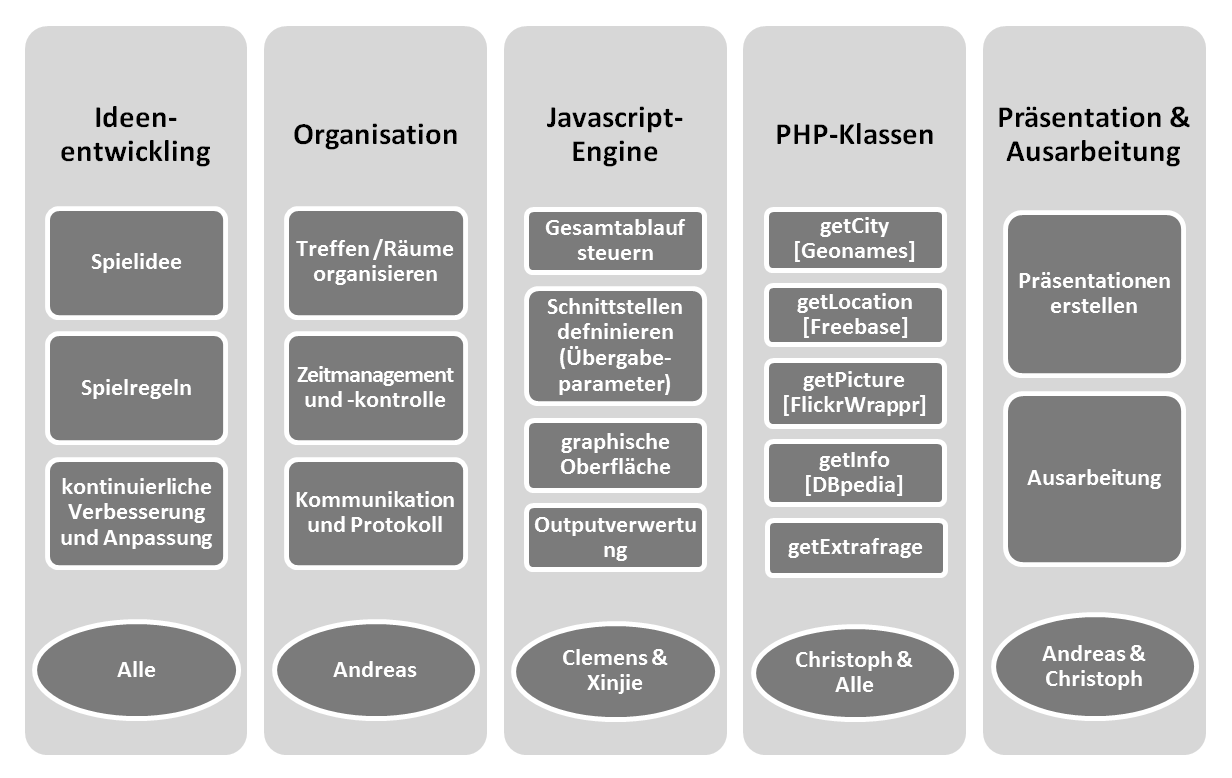
\includegraphics[width=1.0\columnwidth, angle=0]{projektplanung_organigramm_sw.png}
	\caption{Aufteilung der Arbeitspakete}
	\label{img:grafik-dummy}
\end{figure}
Innerhalb des Projektteams wurde für jede Aufgabe Milestones mit Fristen definiert und einer Person direkt zugeordnet.\footnote{Ein Auszug der Liste mit Arbeitspaket, Milestones, Frist und Zuständigkeit ist in der Zwischenpräsentation enthalten.}
\subsection{Evaluierung}
Als vorteilhaft hat sich herausgestellt keine absolute Frist für die Projektidee zu setzen. Aufgrund von Schwierigkeiten mit LOD Datensätzen musste die Idee inkrementell angepasst werden. Die Trennung in Klassen ermöglichte die parallele Ausarbeitung, die mit dem Versionsverwaltungstool Github  effizient ermöglicht wurde. Da trotzdem viel Abstimmung nötig war, stellte das wöchentliche Treffen das Kernelement der Projektdurchführung dar.  Die Aufnahme des Arbeitspakets „Organisation“ war maßgeblich für die effiziente und erfolgreiche Projektkontrolle verantwortlich. Für unseren Einsatzzweck hat sich das Treffen als effektiveres Mittel herausgestellt als eine zu zeitlich determinierte Gesamtplanung innerhalb eines Projektplanungstools.\\\\
Die Unausgeglichenheit der Projektaufgaben aufgrund unterschiedlicher Ausgangspositionen stellte zunächst eine Schwierigkeit dar. Durch klare Verhaltensregeln, spezifische Einarbeitung sowie die Anpassung der Aufgaben an das vorhandene Know-how ist diese Situation nachhaltig verbessert worden.
\newpage
\section{Umsetzung, Softwarepakete und Programm}
\subsection{Schematischer Aufbau, Konzeptskizze}
\begin{figure}[H]
	\centering
	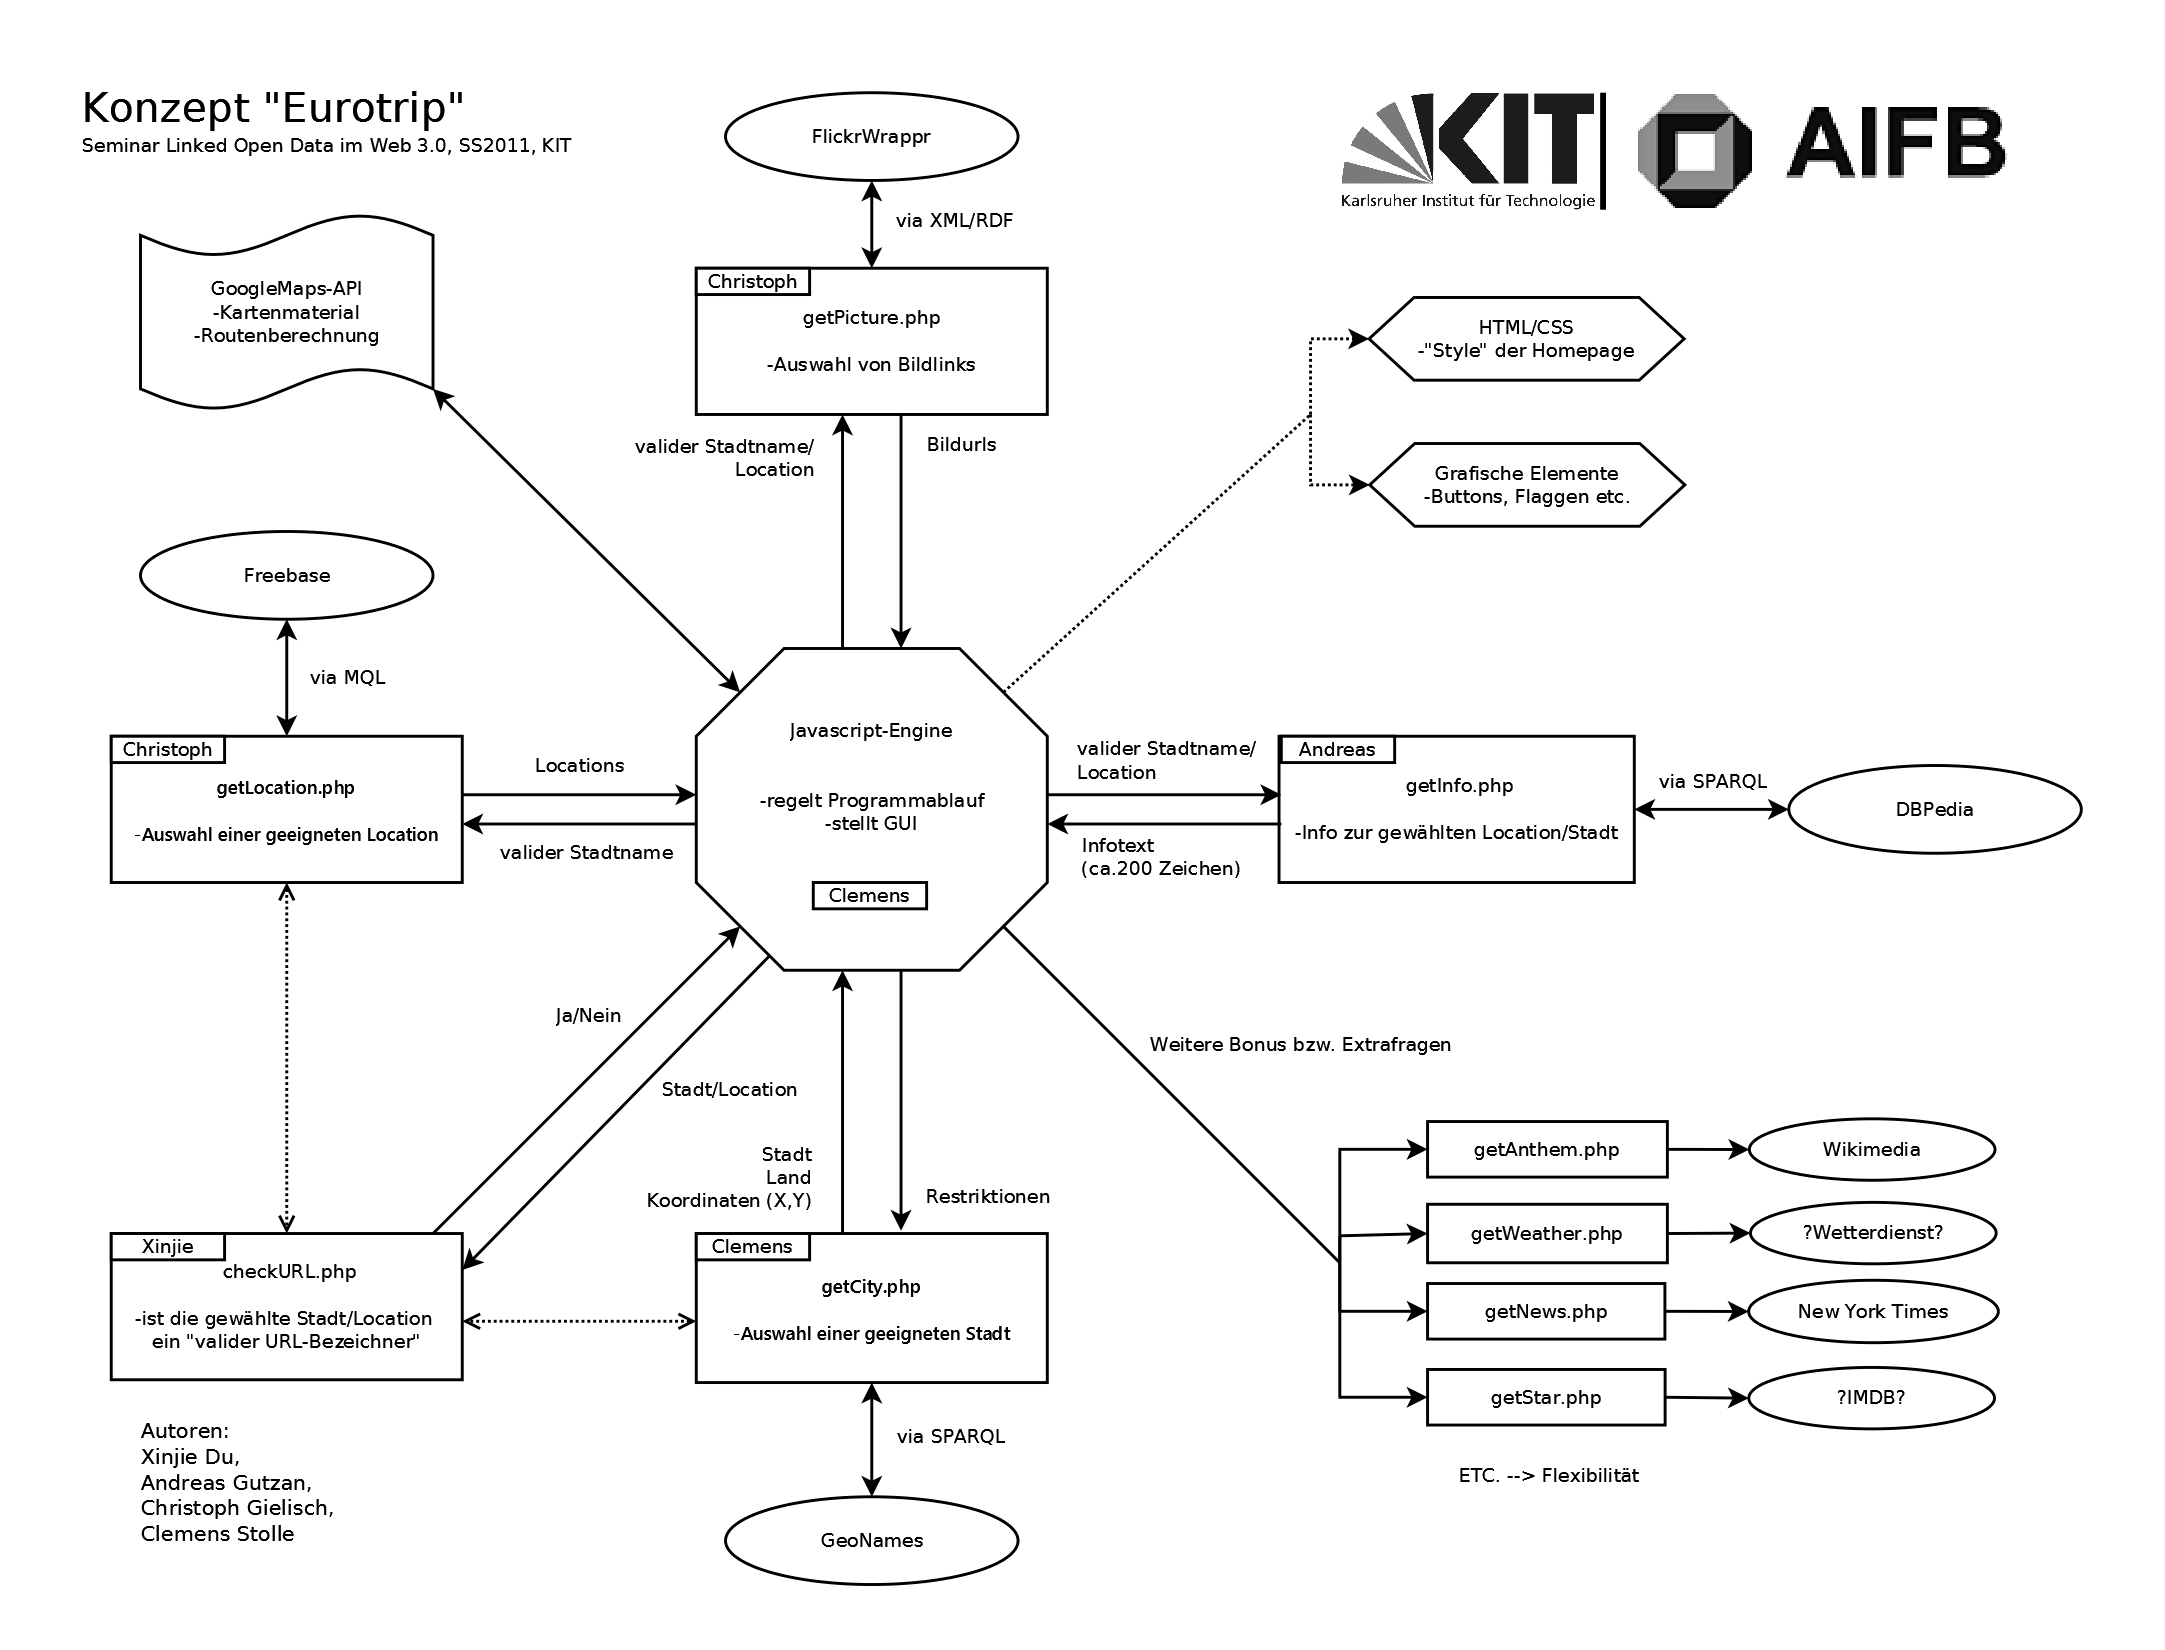
\includegraphics[width=0.5\columnwidth, angle=0]{seminarLOD.png}
	\caption{Konzeptskizze // VERALTET}
	\label{img:grafik-dummy}
\end{figure}
Konzeptionell baut das Programm auf einer zentrierten Struktur auf.
\subsection{Verwendete LOD-Datensätze}
Die verwendeten LOD-Datensätze sind:
\begin{itemize}
\item \textbf{Geonames} wird eingesetzt, um eine Auswahl an Städten zu erzeugen, die der Spieler später dann lokalisieren muss. Diese Datenquelle wurde gegenüber der DBpedia bevorzugt, da bei ihr die Städte klarer strukturiert abgespeichert sind. So fällt die Abfrage der Städte und die Länder in denen diese liegen leichter.
\item Die \textbf{DBpedia} wird gleich an mehreren Stellen im Programm verwendet. Grundsätzlich gilt, dass wenn Namen von Städten, Ländern oder Sehenswürdigkeiten zwischen verschiedenen Programmteilen getauscht werden, dass diese dann mit ihrem DBpedia URI übergeben werden müssen, um valide zu sein. Somit hat man eine gemeinsame Basis, auf der man kommuniziert. Weiterhin werden sowohl der Kurzhinweis als auch die existierende Bonusfrage mit Hilfe der DBpedia generiert. Auch wird dort mit dem dafür zuständigen Tag geprüft, ob eine Sehenswürdigkeit oder Stadt wirklich eine FlickrWrappry-FotoCollection besitzt.
\item \textbf{Freebase} dient vor Allem der Optimierung der Foto-Suchergebnisse. Da sich rein mit einer Stadt getaggte Bilder als teilweise ungenügend herausgestellt haben, wird die Freebase zunächst nach bekannten touristischen Sehenswürdigkeiten der einzelnen Städte abgefragt, da diese i.d.R. bessere Suchergebnisse liefern.
\item Der \textbf{Flickrwrappr} basiert auf einem PHP-Skript der FU Berlin. Man übergibt diesem Skript als Übergabeparameter einen Stadt- oder Sehenswürdigkeitsnamen, welcher dem URI der DBpedia entsprechen sollte. Der Flickrwrappr wiederum antwortet mit Links zu bei Flickr geogetaggten Fotografien als strukturierte Daten in Form einer XML/RDF, die wir wiederum einlesen und verarbeiten.
\item Im Zuge der Bonusfrage können außerdem noch \textbf{weitere Datensätze} in das bestehende Programm integriert werden. Solange diese die gleiche Schnittstelle wie die existierende Bonusfrage benutzen, können sie ohne weitere Probleme in das Programm integriert werden.
\end{itemize}
\subsection{Verwendete Technologien und Frameworks}
Neben dem Linked-Open-Data Ansatzes des Semantic Webs benutzt das Programm selbst noch weitere Technologien und Frameworks.\\\\
Die verwendeten Technologien sind dabei hauptsächlich Javascript für die eigentliche Engine und PHP für die Abfrageklassen. Zur Kommunikation unterhalb dieser Programmteile wird auf AJAX sowie JSON gesetzt. Serverseitig kommt bei uns ein Apache-Server zum Einsatz.\footnote{Einfach mal geraten - NACHPRÜFEN!} Desweiteren wird die gesamte Webseite natürlich in HTML eingebettet und in einem aktuellen Browser über das Internet ausgeführt.\\\\
Als Framework wird vor Allem die "Google Maps API"\footnote{Verlinkung/Quelle} eingesetzt. Sie liefert uns das Kartenmaterial, dessen Anzeige sowie die Abwicklung der Interaktion des Spielers mit ebenjener. Auch die Routenberechnung läuft über dieses Framework.\footnote{Haben wir noch weitere Frameworks im Einsatz?}
\subsection{Dokumentation der Methoden und Funktionen}
\begin{tabular}{|p{3.5cm}|}
\hline
\textsc{getCity.php}
\end{tabular}
\\
\begin{tabular}{|p{2.8cm}|p{2.8cm}|p{5.8cm}|}
\hline
\textsc{Input} & \textsc{Output} & \textsc{Beschreibung}\\
\hline
 - & Array mit: \newline - Stadtname\newline - DBpedia-URI\newline - Land\newline pro Eintrag & Durchsucht Geonames mit gewissen Filterkriterien nach Städten. So wird nach europäischen Städten mit mehr als 400000 Einwohnern gesucht\footnote{Für Deutschland wird dieser Filter auf 250000 abgesenkt}, die nicht in Russland oder der Ukraine liegen.\\
\hline
\end{tabular}
\begin{tabular}{|p{3.5cm}|}
\hline
\textsc{getPictures.php}
\end{tabular}
\\
\begin{tabular}{|p{2.8cm}|p{2.8cm}|p{5.8cm}|}
\hline
\textsc{Input} & \textsc{Output} & \textsc{Beschreibung}\\
\hline
 - & Array mit: \newline - Stadtname\newline - DBpedia-URI\newline - Land\newline pro Eintrag & Durchsucht Geonames mit gewissen Filterkriterien nach Städten. So wird nach europäischen Städten mit mehr als 400000 Einwohnern gesucht\footnote{Für Deutschland wird dieser Filter auf 250000 abgesenkt}, die nicht in Russland oder der Ukraine liegen.\\
\hline
\end{tabular}
\subsection{Stabilität und Verfügbarkeit}
Das Programm an sich läuft trotz seines Prototypen-Status recht stabil. Allerdings ist die Erreichbarkeit von drei Datenquellen für den grundlegenden Ablauf der Fragerunden zwingend erforderlich. Diese sind Geonames, die DBpedia sowie der Flickrwrappr. Ein Ausfall der Freebase würde lediglich die Qualität der Bilder senken, da dann das Heraussuchen von Touristischen Attraktionen wegfallen würde. Sollte einer der Datenbanken der Bonusfragen nicht antworten, wäre ein Fallback auf eine andere Bonusfrage oder das komplette Deaktivieren denkbar. Bei beiden Möglichkeiten ist weiterhin ein stabiler, wenn auch eingeschränkter Betrieb des Programms möglich.\\\\ 
// Hier noch etwas zur Verfügbarkeit der einzelnen Datenquellen
\subsection{Generierung strukturierter Datensätze}
Ein weiterer technischer Aspekt ist die Generierung eigener strukturierter Daten. Dies ist einer der Grundgedanken sowohl des Semantic Webs als auch des Semantic Gamings. Unser Programm ist dabei in der Lage schon rudimentär neu von uns verknüpfte Daten in Kombination mit Daten, die wir durch die Eingabe der Nutzer gewonnen haben, als strukturierte Daten abzuspeichern. Dabei wird für jede Stadt jeweils ein XML-Datensatz angelegt, der dann befüllt wird mit den aktuellen Sehenswürdigkeiten, Bildlinks sowie der vom Nutzer bei genau dieser Kombination erreichten Entfernung zum Zielort.\\\\ Dadurch erschaffen wir eine Datenbank aus der man durch geschicktes Abfragen z.B. mit XPath eine ganz neue Qualität an Information ziehen kann. So sind wir in der Lage bei ausreichend großen Nutzerdateninput durch gemittelte Entfernungen Aussagen über den Bekanntheitsgrad von Städten im Allgemeinen, aber auch deren Sehenswürdigkeiten zu treffen. Denkbar wäre z.B. auch das Blacklisting einzelner Bildlinks als schlechte Fotografien, die eine signifikante Abweichung zu anderen Bildlinks der gleichen Sehenswürdigkeit etc. aufweisen.\\\\
Wir sind damit in der Lage das bei LOD grundlegend heikle Thema der Bewertung von Elementen innerhalb einer Cloud zu verbessern, da man nun mit der Entfernung zumindestens ein Maß für die Bekanntheit dieser Städte uns Sehenswürdigkeiten besitzt.\\\\
Zusammenfassend ist zu sagen, dass die Datensätze so wie wir sie im Moment abspeichern exakt dem entsprechen, was wir zu Beginn der Arbeiten eigentlich als Datenbank gebraucht hätten. Dies dürfte jedoch dem Grundgedanken des Semantic Webs entsprechen, da dieses seine Mächtigkeit ja gerade durch die nahezu unendliche Möglichkeit der Kombination und Verknüpfung von bestehenden und das Einpflegen von neuen strukturierten Daten bezieht.
\subsection{Installation und Betrieb}
Das Spiel selbst benötigt keine clientseitige Installation. Einzig ein funktionierender, aktueller Browser, der in der Lage ist Javascript auszuführen, ist von Nöten. Der Start erfolgt durch Ansteuerung der Webadresse.\\\\
Für den Betrieb des Spiels ist der Anbieter des Porgramms allerdings gezwungen einen Webserver zu betreiben. Dieser muss in der Lage sein PHP-Code zu interpretieren und so die nötigen Abfragen auf die verschiedenen Datenquellen auszuführen.
\newpage
\section{Lessons learned}
\subsection{Reflektion der Projektplanung}
\subsection{Erkenntnisse}
\subsection{Vor- und Nachteile von Linked Open Data}
\newpage
\section{Fazit}
\subsection{Zusammenfassung}
\subsection{Stärken und Schwächen}
\subsection{Ausblick}

  
% das ist wohl jetzt das Ende des Dokumentes
\end{document}